\sectionmark{Gärung I}

\section{Gärung I}
\begin{enumerate}
	\item Was versteht man unter einer klassischen Gärung und wie unterscheidet sie sich von Atmungsprozessen?
	
		Als Gärung bezeichnet man eine intern ausbalancieten Oxidations-Reduktion.
		Die klassischen Charakteristiken einer Gärung sind:
		\begin{itemize}
			\item keine externen e\textsuperscript{-}-Akzeptoren
			\item keine direkte mit Substratoxidation gekoppelte Elektronentransport-Phosphorylierung.
			\item organische Verbindungen als Substrate
		\end{itemize}

	\item Benennen Sie Gärungsprodukte und Organismen, die diese Produkte produzieren.
		
		In Tabelle \ref{tab:gaerungsprodukte} sind einige Organismen und ihre Gärungsprodukte aufgeführt.
		Zentralles Intermediat ist in den aufgeführten Vorgängen immer Pyruvat.
		\begin{table}[h!]
		\begin{center}
		\begin{tabular}{l l} 
		\toprule
			Organismengruppe			&	Gärungsprodukt\\
			\midrule
			Milchsäurebakterien		&	Lactat\\
			Hefen							&	Ethanol\\
			Propionibakterien			&	Propionat\\
			Coli-Aerogenes-Gruppe	&	Butandiol\\
			Clostridien					&	2-Propanol, Butanol\\
		\bottomrule
		\end{tabular}
		\caption{Verschiedenen Mikroorganismen und ihre Gärungsprodukte.}
		\label{tab:gaerungsprodukte}
		\end{center}
		\end{table}

	\item Wieso muss bei einer Gärung die Wasserstoffbilanz ausgeglichen werden?
		
		IMHO:\\
		Da die Elektronen sonst nicht auf einen Carrier übertragen werden können,
		da sie vom \ce{H+} gebunden werden.		%TODO- verifizieren!

	\item Auf welchen Wegen kann der initiale Glucoseabbau bei unterschiedlichen Gärungen erfolgen (mit Beispielen)?
	
		In Tablle \ref{tab:fermenterglyoklyse} sind einige Organismengruppen und ihre Glukoseabbauwege aufgeführt.	
		\begin{table}[h!]
		\begin{center}
		\begin{tabular}{l l} 
		\toprule
			Organismengruppe			&	Glykolyse-Weg\\
			\midrule
			``die Meisten Fermetierer''		&	Embden-Meyerhof-Weg\\
			Zymomonas							&	Entner-Doudorof-Weg\\
			hetero-fermentative Milchsäure G.			&	Phosphoketolase\\
%			andere					&	Oxidativer Pentosphosphat-Weg\\		%geht nicht aus Folie hervor, Gaerung1,S.4
		\bottomrule
		\end{tabular}
		\caption{Verschiedenen Mikroorganismen und ihre Gyloklyse-Wege.}
		\label{tab:fermenterglyoklyse}
		\end{center}
		\end{table}

	\item Geben Sie Beispiele für C-Quellen, die von Saccharomyces fermentiert, veratmet, bzw. nicht verwertet werden können.

	Glucose (\ce{C6H12O6}) kann sowohl veratmet als auch vergärt werden.	
		\begin{description}
			\item[Atmung] \hfill\\
				\ce{C6H12O6} + \ce{602} \textrightarrow \ \ce{6CO2} + \ce{6H2O} \hfill 32-36 ATP	
			\item[Gärung] \hfill\\
				\ce{C6H12O6} \textrightarrow \ \ce{2CO2} + 2\ce{CH3}-\ce{CH2}-\ce{OH} \hfill 2 ATP
		\end{description}

	\item Welche Enzyme werden für die Alkoholische Gärung benötigt und welches ist das Schlüsselenzym?

		Für die Alkoholische Gärung werden sowohl im Embden-Meyerhof-Parnas-Weg,
		als auch im Entner-Doudoroff-Weg folgende Enzyme benötigt:
		\begin{itemize}
			\item Pyruvat-Decaboxylase
			\item Ethanol-Dehydrogenas
		\end{itemize}
		
	\item Bei welchen Schritten werden bei der Alkoholischen Gärung ATP gebildet oder Reduktionsäquivalente verbraucht?
		%TODO brock lookup	
	\item Wie und warum unterscheidet sich die ATP-Ausbeute bei den alkoholischen Gärungen von Zymomonas mobilis und Saccharomyces cerevisiae?
	\item Welche Standorte besiedeln Milchsäurebakterien?
		
		Milchsäurebakterien finden sich in folgenden Habitaten:
		\begin{itemize}
			\item Pflanzen
			\item Milch, Milchprodukte
			\item Darm
			\item Schleimhäute
			\item Hautflora
		\end{itemize}

	\item Im Rahmen welcher Gärung taucht Methylmalonyl-CoA als Zwischenprodukt auf?
		
		Während des Fruktose-1,6-bisphosphat-Weges.

	\item Was ist das Schlüsselenzym der Milchsäuregärung?

		Kandidaten:
		\begin{itemize}
			\item Laktat-Dehydrogenase
			\item Phosphoketolasee
		\end{itemize}

	\item Benennen Sie Charakteristika von Bifidobakterien?
		
		Der Name der ergibts sich aus ihrer ``gespaltenen'', V- bzw. Y-Form.
		Ihr Habitat ist die Darmflora von Säuglingen,
		wohin sie durch die Muttermilch gelangen.
		In Kuhmilch sind sie jedoch nicht vorhanden.
		Es handelt sich um nicht aerotolerante Bakterien,
		die eine \ce{CO2} Atmosphäre benötigen.
		Bifidobakterien gären über den Phosphoketolase-Nebenweg.

	\item Wo verzweigen sich die Wege der homo- und der heterofermentativen Milchsäuregärung?
		
		Bei der Umsetzung von Glucose-6-Phosphat,
		welches bei der homo-fermentativen Milchsäuregärung zu Fructose-6-Phosphat umgesetzt wird
		und bei der hetero-fermentativen Milchsäuregärung zu 6-Phosphogluconat.

	\item Wie kommen die Löcher in den Emmentaler Käse?

		Die Löcher entstehen durch die \emph{Propionibakterien}.
		Sie vergären das Laktat auch zu \ce{CO2} (s.u.),
		welches die Löcher bedingt.
		\emph{Propionibakterien} sind gram-positive und	aerotolerant.
		Sie besiedeln den Pansen und Darm von Wiederkäuern und bauen Glukose über den
		Fruktose-1,6-bisphosphat-Weg ab, die weiter Gärung erfolgt mit:
		
		3 Laktat \textrightarrow \ 2 Propionat + 1 Acetat + \ce{CO2} + \ce{H2O}

	\item Nennen Sie Arten der Enterobacteriaceae.

		Die Enterobakterien sind gram-negative Stäbchenbakterien.
		Sie Sind peritrich begeißelt und somit beweglich.

		\begin{description}
			\item[E. coli] Darm
			\item[Enterobacter aerogenes] Boden
			\item[Erwinia] Pflanzen (pathogen)
		\end{description}

	\item Welches Verhältnis haben Enterobacteriaceae zum Sauerstoff?

		Seit dem sie sich von 2 Jahren getrennt haben, wegen der Affäre des Sauerstoffs mit einem Radikalen,
		versuchen sie einen freundschaftliche Kontakt zu halten.
		%scnr,dunno

	\item Welche Gärprodukte werden von Enterobakterien gebildet?

		Folgenden Gärprodukte werden von Enterobakterien aus Hexosen gebildet:
		\begin{itemize}
			\item Ethanol
			\item 2,3-Butandiol
			\item Succinat
			\item Lactat
			\item Acetat
			\item Diacetyl
			\item Formiat
			\item \ce{H2}
			\item \ce{CO2}
		\end{itemize}

	\item Welche zwei Gärungstypen werden bei der gemischten Säuregärung unterschieden? Benennen sie hierfür repräsentative Vertreter!
	
		\emph{E. coli} verwendet einen Gärungstyp bei dem viel Säure und kein 2,3-Butandiol endsteht.
		Das Verhältnis von sauren Gärprodukten zu neutralen ist hier 4:1.
		Beim  zweiten Gärungstypen beträgt das Verhältnis 1:6.
		\emph{Enterobacter} und \emph{Klebsiella} beispielsweise,
		erzeigen hingegen wenig Säure und 2,3-Butandiol.

	\item Wie entstehen bei der gemischten Säuregärung Formiat, Wasserstoff und Kohlendioxid?
		
		Nach der Glykolyse bleibt Phosphoenolpyruvat über.
		Dieses wir unter ATP gewinn zu Pyruvat.
		Pyruvat kann nun mit der Pyruvat-Formiat-Lyase ind Acetyl-CoA und Formiat umgesetzt werden.
		Durch die weiter umsetzung mit Formiat-Hydrogen-Lyase endsteht \ce{CO2} und \ce{H2}.
		Siehe auch Abbildung \ref{fig:butandiolgaerung}.

	\item Wie entsteht 2,3-Butandiol und welche Enterobakterien produzieren es?

		Wie in Abbildung \ref{fig:butandiolgaerung} zu sehen ist,
		endsteht auch 2,3-Butandiol ursprünglich aus Pyruvat.
		Die Umsetzung er folgt dann im letzten Schritt mit 2,3-Butandiol-Dedhydrogenase
		aus Acetoin und NADH.
		
		\begin{figure}[ht]
		\leavevmode
		\begin{center}
		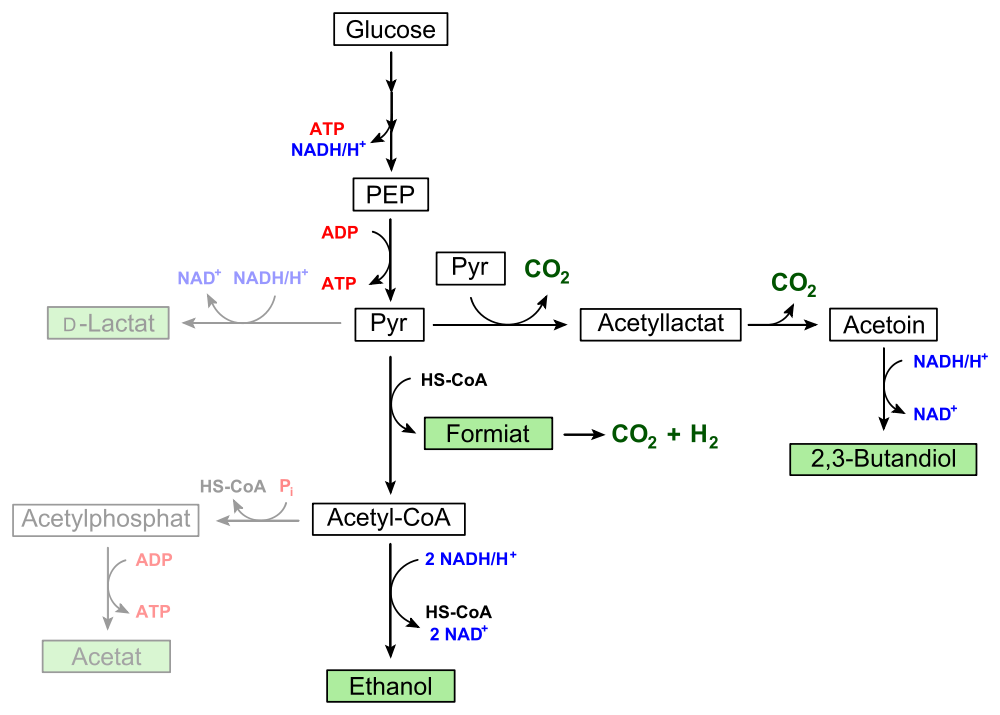
\includegraphics[scale=0.32]{./pictures/butandiolgaerung_1000}
		\end{center}
		\caption{\slshape{Butandiolgärung}}
		\label{fig:butandiolgaerung}
		%von wikipedia
		\end{figure}

		Die vorherigen Schritt sind:
		\begin{enumerate}[label=\arabic*)]
			\item Pyruvate \textrightarrow Hydroxyethyl-Thiamin pyrophosphat (HTPP)	\\
			\hfill(\ce{CO2}-Abaspaltung)
			\item Acetolacata-Synthase(HTPP + Pyruvat) \textrightarrow \begin{math}\alpha\end{math}-Acetolactat \\
			\hfill(TPP-Abspaltung)
			\item Acetolactat-Decarboxylase(\begin{math}\alpha\end{math}-Acetolactat) \textrightarrow Acetoin \\
			\hfill(\ce{CO2}-Abaspaltung)
			\item 2,3-Butandiol-Dehydrogenynase(Acetoin + NADH) \textrightarrow 2,3-Butandiol
		\end{enumerate}
		Acetoin wird auch mit der Acetoin-Dehydrogenase zu Diacetyl umgesetzt.
		Dabei wird NADH frei, 
		welches mit der 2,3-Butandiol-Dehydrogenynase und Acetoin zu 2,3-Butandiol umgesetzt werden kann.

		Die Butandiolgärung wird von z.B. von \emph{Klebsiella oxytoca} und \emph{Enterobacter} durchgeführt.

	\item Unter welchen Bedingungen wird die Bildung von 2,3-Butandiol begünstigt?
	
		Acetat stimuliert die Bildung von 2,3-Butandiol.

	\item Wie verteilen sich die Produkte bei der Vergärung von Glucose durch \emph{E. coli} bei Wachstum unter alkalischen bzw. sauren Bedingungen?
		
		Unter alkalischen Bedingungen endsteht Ameisensäure,
		welche unter sauren Bedingungen kaum endsteht.
		Dafür wird im Sauren deutlich mehr Gas in Form von \ce{CO2} und \ce{H2} erzeugt.

	\item Wie entsteht Succinat bei anaeroben Wachstum von Escherichia coli? Handelt es sich um einen Atmungs- oder Gärungsprozess?
		
		Succinat endsteht als Gärungsprodukt.
		Phosphoenolpyruvat wird unter Anlagerung von \ce{CO2} mit der PEP-Caboxylase zu Oxalacetat umgesetzt.
		Mit der Malat-Dehydogenase wird das Oxalacetat zu Malat umgesetzt.
		Durch die Fumarase(FumB) endsteht aus Malat Fumerate,
		welches unter Anlagerung von \ce{H2} mit der Fumarat-Reduktase zu Succinat wird.
\end{enumerate}
